%SourceDoc ../YourName-Dissertation.tex
% \vspace*{-80mm}
\chapter{Background} \label{chapter1:Background}

\section{\sloppy Gaussian Processes}

Consider a \emph{spatial stochastic process}~\cite{gelfand2010handbook} $\{Y(\bm{s}): \bm{s} \in \mathcal{D} \subseteq \mathbb{R}^d\}$ that varies over some continuous spatial domain $\mathcal{D}$. We will focus on the most common case for spatial statistics, where the dimension is $d = 2$, although the methods presented here are valid for any $d$.  For a finite collection of spatial locations $\{\bm{s}_1, \dots, \bm{s}_n\} \subset \mathcal{D}$, $\bm{Y} = (Y(\bm{s}_1), \dots, Y(\bm{s}_n))^T$ is a random vector where each element is associated with one location. The multivariate distribution of $\bm{Y}$ contains information about the spatial dependencies between all $n$ locations.

The distribution of the process $\{Y(\bm{s})\}$ may be described through its finite-dimensional joint distributions
\begin{equation} \label{eq:joint}
F(y_1, \dots, y_n; \bm{s}_1, \dots, \bm{s}_n) = P(Y(\bm{s}_1) \leq y_1, \dots, Y(\bm{s}_n) \leq y_n)
\end{equation}
for every value of $n$ and every set of $n$ spatial locations in $\mathcal{D}$. A \emph{Gaussian process} is a special case in which every distribution in \eqref{eq:joint} is multivariate normal~\cite{gelfand2010handbook}. As a result, the distributions are all completely characterized by their means and covariance matrices, which makes Gaussian processes much easier to work with than non-Gaussian spatial stochastic processes.

% section gaussian_processes (end)

\section{Stationarity and Isotropy} % (fold)
\label{sec:stationarity_and_isotropy}

Throughout this work we will be making two key assumptions:  \emph{stationarity} and \emph{isotropy}. A stationary Gaussian process is one that does not vary with spatial shifts. That is, for any lag vector $\bm{h} \in \mathbb{R}^d$,
\[
E[Y(\bm{s})] = E[Y(\bm{s} + \bm{h})] = \bm{\mu}
\]
and
\[
\textrm{Cov}(Y(\bm{s}), Y(\bm{s} + \bm{h})) = \textrm{Cov}(Y(\bm{0}), Y(\bm{h})) = C(\bm{h}).
\]
Here $C(\bm{h})$ is called the \emph{covariance function}.

For isotropic Gaussian processes, the covariance function depends on $\bm{h}$ only through its magnitude $||\bm{h}||$. In this setting, we can express the covariance function simply as $C: [0, \infty) \to \mathbb{R}$. If we assume without loss of generality that the process is standardized, we can further stipulate that $C(0) = 1$ and $E[Y(\bm{s})] = 0$ for all $\bm{s} \in \mathcal{D}$.

% Define $\mathcal{C}_d$ as the set of all continuous isotropic covariance functions in $d$ dimensions. Further define $\mathcal{C}_\infty = \bigcap_{d=1}^\infty \mathcal{C}_d$ as the set of all functions that are valid isotropic covariance functions in \emph{all} dimensions. It can be shown~\cite{Stein1999}~\cite{schoenberg1938metric} that
% \[
% 	\mathcal{C}_1 \supseteq \mathcal{C}_2 \supseteq \cdots \supseteq \mathcal{C}_\infty
% \]
% and that a function $C(h)$ is in $\mathcal{C}_\infty$ if and only if it can be written in the form
% \[
% 	C(h) = \int_0^\infty \exp(-h^2u^2) \; dG(u)
% \]
% for some $G$ bounded and non-decreasing on $[0, \infty)$~\cite{Stein1999}.

% section stationarity_and_isotropy (end)

\section{Covariance Function Estimation} % (fold)
\label{sec:covariance_function_estimation}

Because Gaussian processes are completely characterized by their mean and covariance functions, estimating $C$ given a collection of observations $\{y_1, \dots, y_n\}$ is a topic of great interest~\cite{ver1993multivariable}~\cite{banerjee2014hierarchical}. The problem of estimating $C$ differs from the general problem function estimation because only a restricted class of functions will produce a valid Gaussian process. In particular, $C$ must belong to the class of \emph{positive definite functions}, which is defined as the set of all functions $C$ such that
\[
  \sum_{i=1}^n \sum_{j=1}^n a_i a_j C(\bm{s_i}\bm{s}_j) > 0
\]
for any $n$, any $\{\bm{s}_1, \dots, \bm{s}_n\} \in \mathcal{D}$, and any $a_1, \ldots, a_n \in \mathbb{R}$. This condition guarantees that the joint distribution of any finite collection of observations $\{Y(\bm{s}_1), \ldots, Y(\bm{s}_n)\}$ has a positive definite covariance matrix. This turns out to be a strong restriction, and it is very difficult in general to directly estimate $C$ in such a way that forces positive definiteness.

The classical approach to overcoming this difficulty is to select a parametric family of covariance functions that is known to be positive definite for a given range of the parameters, and to estimate the parameters using moment- or likelihood-based methods\cite{gelfand2010handbook}. A popular choice of parametric families is the \emph{Mat\'{e}rn} class of functions~\cite{handcock1994approach}, which take the form
\begin{equation} \label{eq:matern}
C(h) = \frac{\sigma^2}{2^{\nu - 1}\Gamma(\nu)} \left( \frac{2\nu^{1/2}h}{\rho} \right)^{\nu} \mathcal{K}_{\nu} \left( \frac{2\nu^{1/2}h}{\rho} \right), \qquad \sigma^2, \nu, \rho > 0,
\end{equation}
where $\mathcal{K}_\nu$ is a modified Bessel function of the third kind. This is a three-parameter family, with $\sigma$ controlling the marginal variance, $\rho$ controlling the range of correlation, and $\nu$ controlling the smoothness of the sample paths. All functions in this class are positive definite for observations in any dimension~\cite{Stein1999}. Some examples of Mat\'ern covariance functions are shown in Figure~\ref{fig:matern_examples}.


\begin{figure}[!htb]
	\centering
	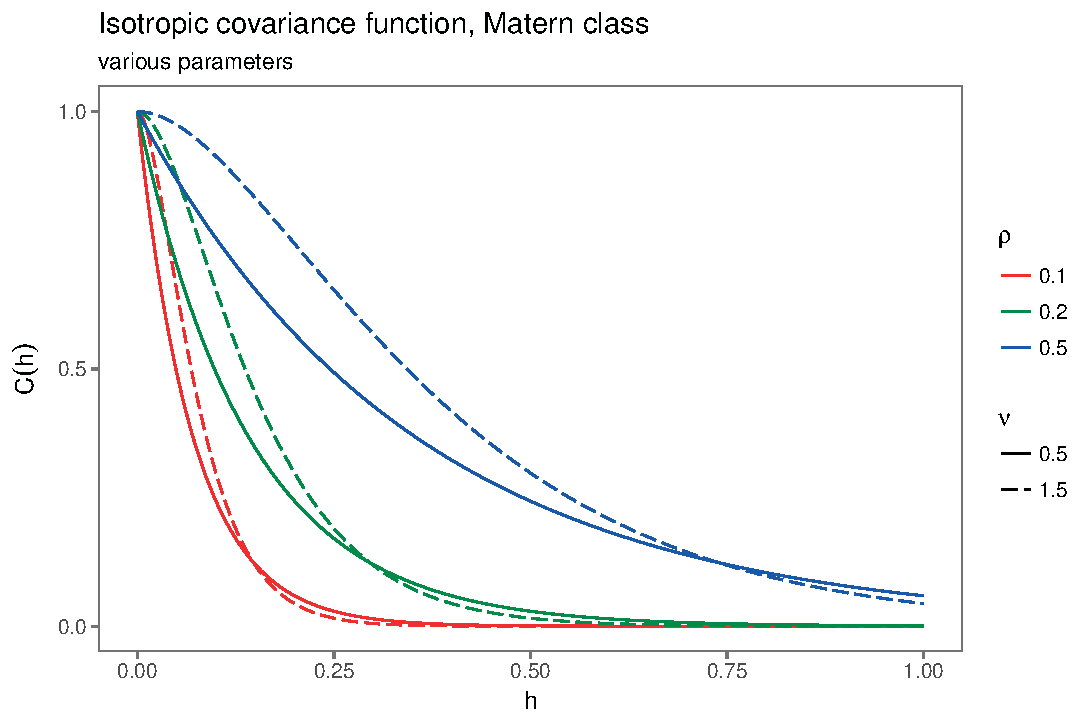
\includegraphics[width=0.95\textwidth]{matern_examples.pdf}
	\caption{\small The Mat\'ern isotropic covariance function \eqref{eq:matern} for various choices of $\nu$ and $\rho$, each with $\sigma^2 = 1$.}
	\label{fig:matern_examples}
\end{figure}


Another positive definite family, which we will use in examples below, is the \emph{exponentially damped cosine} class, 
\begin{equation} \label{eq:dampedcos}
	C(h) = \sigma^2 \exp \left( -\tau \frac{h}{\lambda} \right) \cos \left( \frac{h}{\lambda} \right), \qquad \tau \geq \frac{1}{\tan \frac{\pi}{2d}}, \quad \sigma^2,\lambda > 0.
\end{equation}
Unlike the Mat\'ern class, the damped cosine class allows for negative correlations at certain distances. This non-monotonic behavior is known in geostatistical applications as a \emph{hole effect}~\cite{Ye2015}, and is shown in Figure~\ref{fig:dampedcos_examples}. The restriction on $\tau$ that depends on $d$ is necessary for functions of this form to be positive definite. %Note, however, that $\tan(\pi/2d) \to 0$ as $d \to \infty$, so this set of functions is not a member of $\mathcal{C}_\infty$. 
The damped cosine family is not nearly as commonly used as the Mat\'ern family, but it is useful in some applications because allows for stochastically periodic behavior as well as negative correlations, which a Mat\'ern family cannot capture. However, it does not share the attractive feature of the Mat\'ern family that the smoothness of the process (i.e. the degree of differentiability) is controlled by a parameter that can be estimated from the data. The smoothness is closely related to the local behavior of the process, which crucial to obtaining good performance when interpolating the process at unobserved locations~\cite{Stein1999}.

\begin{figure}[!htb]
	\centering
	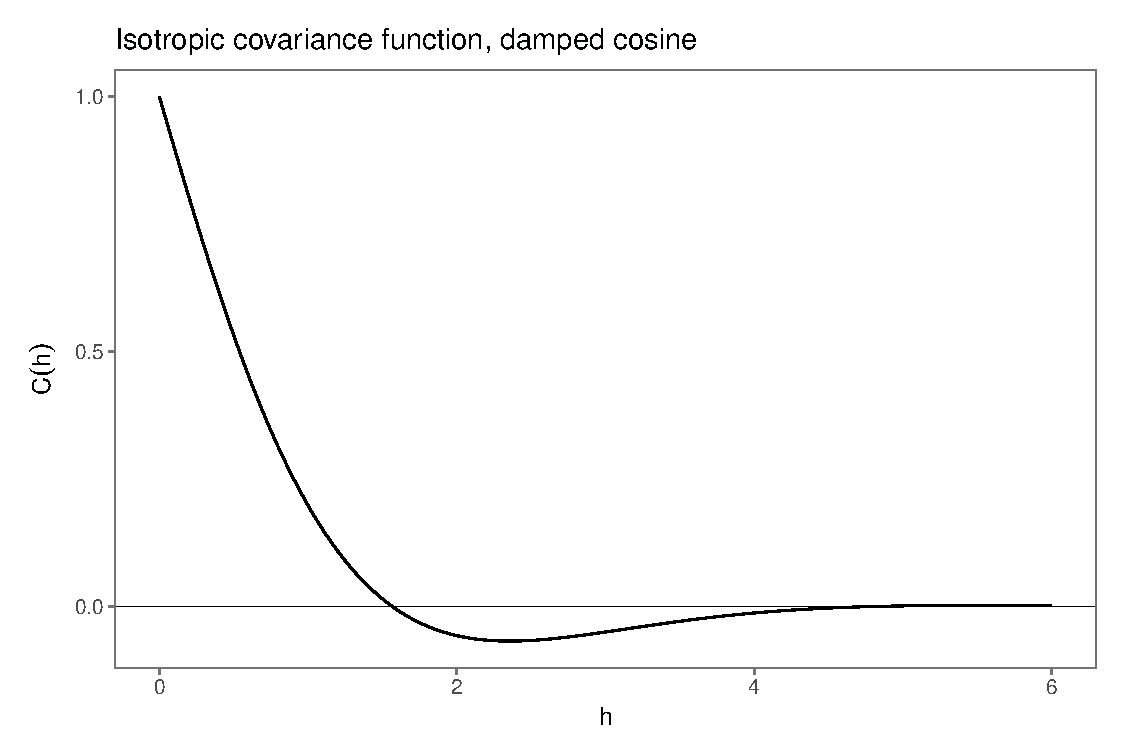
\includegraphics[width=0.95\textwidth]{dampedcos_examples.eps}
	\caption{\small The damped cosine isotropic covariance function \eqref{eq:dampedcos} for $\tau = 1$, $\lambda = 1$, and $\sigma^2=1$. Notice that $C(h) < 0$ for certain values of $h$.}
	\label{fig:dampedcos_examples}
\end{figure}

The strategy of fitting the data to a parametric family of covariance functions can produce a good estimate if the true covariance structure is close to the structure assumed by the choice of parametric family. However, there is no guarantee that this will be the case. For instance, if the true covariance contains a hole effect, there is no way for a Mat\'ern model to capture it since $C(h) > 0$ for all $h$. More preferable would be a flexible method that allows the spatial dependence in the data itself, rather than the choice of parametric family, to determine the shape of $C$.

% subsection estimating_the_covariance_function (end)

\section{The Spectral Domain and Bochner's Theorem} % (fold)
\label{sec:bochner_s_theorem}

The method proposed in this work takes advantage of the result from Bochner~\cite{bochner1955harmonic} which says that a real-valued continuous function $C$ is positive definite if and only if it is the Fourier transform of a symmetric, non-negative, finite measure $F$ on $\mathbb{R}^d$. That is, $C$ is positive definite if and only if
\begin{equation} \label{eq:bochner}
C(\bm{h}) = \int_{\mathbb{R}^d} \exp(i \bm{h}^T \bm{\omega}) \; dF(\bm{\omega}),
\end{equation}
In most circumstances, the measure $F$ has a Lebesgue density, $f(\bm{\omega})$, which is referred to as the \emph{spectral density}~\cite{gelfand2010handbook}.  Furthermore, because we are assuming that the Gaussian process described by $C$ is isotropic, $C$ is a function of a scalar $h$, so that
\begin{equation} \label{eq:bochner2}
C(h) = \int_{\mathbb{R}} \cos(h\omega) \; f(\omega) \; d\omega.
\end{equation}
Stein~\cite{Stein1999} argues that for Gaussian process covariance functions to be realistic models for spatial phenomena, spectral densities $f(\omega)$ must be heavy tailed.

The relationship between the covariance function and the spectral density given in \eqref{eq:bochner2} suggests us an alternative way to estimate the covariance function $C(h)$. If we can estimate the the symmetric spectral density $f(\omega)$, then we are assured that the corresponding covariance function $C(h)$ is positive definite.  Flexibly modeling $C(h)$ directly is difficult because of the restriction of positive definiteness, but flexibly modeling $f(\omega) $ is easy because it can be any symmetric density.

There have been previous approaches for non- and semi-parametric methods that estimate $C(h)$ using the spectral domain. Most closely related to our approach is that of Im, Stein, and Zhu~\cite{IM2007}, who estimate the spectral density using a combination of cubic B-splines with an explicitly specified algebraically decaying tail.   Constraints are placed on the spline coefficients to ensure that the spectral density is non-negative, thereby resulting in a covariance function is positive definite.  Im, Stein, and Zhu use the fact that when under isotropy, \eqref{eq:bochner} can be written as an integral over only one dimension,
\[
	C(h) = 2^{(d-2)/2}\Gamma(d/2) \int_0^\infty (hu)^{-(d-2)/2} J_{(d-2)/2}(hu) \; dG(u),
\]
where $J_\nu(\cdot)$ is the Bessel function of the first kind of order $\nu$. The spline-based spectral density is transformed into a covariance function using numerical integration, which is then used to construct the likelihood of the spline coefficients given the data.  This likelihood is be maximized over the constrained set of spline coefficients to produce $d\hat{G}(u)$, and hence $\hat{C}(h)$.  Our method follows this same concept, with some notable differences outlined in Chapter~\ref{chapter2:Procedure}.

Another, earlier method was put forth by Hall, Fisher and Hoffmann~\cite{Hall1994}. They proposed a multistep process which begins with a kernel estimate of the covariogram. Because the kernel estimate is not necessarily positive definite, they numerically compute its Fourier transform, set all frequencies beyond the first negative value to zero, and then numerically Fourier transform it back to the spatial domain. In the simulation study in Chapter~\ref{chapter3:Simulation-Study}, we compare our method to the one from Hall et al., as well as to the Mat\'ern model fit by maximum likelihood.

In Chapter~\ref{chapter4:Data-Application}, we apply our method to data from a paper by Singh et al. \cite{Singh2014}, where we model the thickness of a thin film semiconductor in a photovoltaic cell as a Gaussian process. The results are discussed in Chapter~\ref{chapter5:Conclusions}, as well as possibilities for improvements and future directions for this work.

% section bochner_s_theorem (end)
